%@descr: wzór sprawozdania, raportu lub pracy - nadaje się do przeróbek
%@author: Maciej Komosiński

\documentclass{article} 
\usepackage{polski} %moze wymagac dokonfigurowania latexa, ale jest lepszy niż standardowy babel'owy [polish] 
\usepackage[utf8]{inputenc} 
\usepackage[OT4]{fontenc} 
%\usepackage{gensymb}
\usepackage{graphicx,color} %include pdf's (and png's for raster graphics... avoid raster graphics!) 
\usepackage{url} 
\usepackage[pdftex,hyperfootnotes=false,pdfborder={0 0 0},colorlinks=true, linkcolor=blue]{hyperref} %za wszystkimi pakietami; pdfborder nie wszedzie tak samo zaimplementowane bo specyfikacja nieprecyzyjna; pod miktex'em po prostu nie widac wtedy ramek


% Zmiana rozmiarów strony tekstu
\addtolength{\voffset}{-1cm}
\addtolength{\hoffset}{-1cm}
\addtolength{\textwidth}{2cm}
\addtolength{\textheight}{2cm}

%bardziej zyciowe parametry sterujace rozmieszczeniem rysunkow
\renewcommand{\topfraction}{.85}
\renewcommand{\bottomfraction}{.7}
\renewcommand{\textfraction}{.15}
\renewcommand{\floatpagefraction}{.66}
\renewcommand{\dbltopfraction}{.66}
\renewcommand{\dblfloatpagefraction}{.66}
\setcounter{topnumber}{9}
\setcounter{bottomnumber}{9}
\setcounter{totalnumber}{20}
\setcounter{dbltopnumber}{9}

% własny bullet list z malymi odstepami
\newenvironment{tightlist}{
\begin{itemize}
  \setlength{\itemsep}{1pt}
  \setlength{\parskip}{0pt}
  \setlength{\parsep}{0pt}}
{\end{itemize}}

%obrazkow szukamy w nastepujacym katalogu:
\graphicspath{{pics/}}



%\title{Sprawozdanie z laboratorium:\\Metaheurystyki i Obliczenia Inspirowane Biologicznie}
%\author{}
%\date{}


\begin{document}

\thispagestyle{empty} %bez numeru strony

\begin{center}
{\large{Sprawozdanie z laboratorium:\\
Informatyka w Medycynie\\
(szablon)}}

\vspace{3ex}

Część I: Symulator tomografu komputerowego
%Część II: Algorytmy optymalizacji lokalnej i globalnej, problem QAP
%Część III: Eksperyment: ... (prezentację można zrobić w LaTeX - służy do tego klasa "beamer")

\vspace{3ex}
{\footnotesize\today}

\end{center}


\vspace{10ex}

Prowadzący: mrg inż. Iwo Błądek

\vspace{5ex}

Autorzy:
\begin{tabular}{lllr}
\textbf{Sebastian Firlik} & inf122485 & I2 & sebastian.firlik@student.put.poznan.pl \\
\textbf{Piotr Hankiewicz} & inf1225** & I2 & MAIL \\
\end{tabular}

\vspace{5ex}

Zajęcia piątkowe, 11:45.

\vspace{35ex}

\noindent Oświadczam/y, że niniejsze sprawozdanie zostało przygotowane wyłącznie przez powyższych autora/ów,
a wszystkie elementy pochodzące z innych źródeł zostały odpowiednio zaznaczone i~są cytowane w bibliografii.  

\newpage



\section*{Udział autorów (jeśli $>1$)}
\begin{tightlist}
\item JK zaimplementował..., przeprowadził eksperyment..., opisał..., przygotował...
\item EK zaimplementowała..., przeprowadziła eksperyment..., opisała..., przygotowała...
\end{tightlist}



\section{Wstęp}

Naszym zadaniem było stworzenie aplikacji desktopowej w wybranej technologii i zaimplementowanie w niej symulacji dwuwymiarowego tomografu komputerowego. Wszystkie wymagania zostały wypunktowane \href{https://www.cs.put.poznan.pl/ibladek/students/iwm/0_projekt_wspolny_Tomograf.pdf}{tutaj}. Do stworzenia naszej aplikacji użyliśmy:
\begin{tightlist}
\item języka Python 3,
\item środowiska PyQt5 do stworzenia interfejsu okienkowego,
\item bibliotek dostępnych w języku Python (matplotlib, numpy, pyDicom...)
\end{tightlist}

Jedynie do obsługi zapisu do formatu DICOM użyliśmy gotowej biblioteki ze względu na trudność manipulacji danymi w tym formacie. Wszystkie obliczenia, zarówno podczas generacji sinogramu, jak i przejściu do obrazu wynikowego, a także obrót emitera i detektorów w funkcji kąta zamodelowaliśmy samodzielnie.

\begin{figure}[!htbp]
\begin{center}
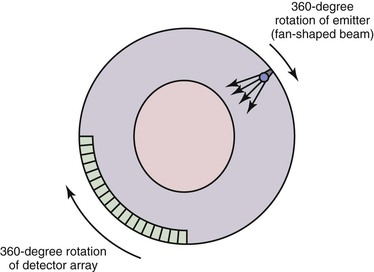
\includegraphics[width=0.8\textwidth]{tomograf.jpg}
\end{center}
\caption{Schemat działania tomografu}
\label{fig:1Tdelta}
\end{figure}

Na Rysunku 1 widzimy, jak działa nasz tomograf komputerowy - jeden emiter obraca się o $360 ^{\circ}$, wysyła promieniowanie rentgenowskie przez badany obiekt i każda wiązka trafia na odpowiedni detektor. W naszej symulacji, przy pomocy algorytmu Bresenhama tworzymy dyskretną linię, prowadzącą od emitera do detektora przez obraz i sumuje jasności pikseli na tej drodze. W ten sposób, na każdej ścieżce emiter-detektor, dla każdego możliwego kąta obrotu emitera, otrzymujemy \textbf{sinogram}, czyli pośredni etap wizualizacji badanego obiektu. Nie podlega on żadnej analizie diagnostycznej. Następnie w wyniku operacji odwrotnej (Odwrotna Dyskretna Transformata Radona) otrzymujemy obraz wynikowy. 

ODTR polega na tym, że z każdym kątem obrotu $\alpha$ i każdą parą emiter-detektor sprzężona jest suma jasności pikseli na ich drodze. Teraz na każdym pikselu, znajdującym się na tej drodze, zostawiamy średnią jasność piksela, wynikającą z odpowiedniej sumy z sinogramu. Po iteracyjnym odtworzeniu obrazu, bez nałożonego filtrowania widzimy niedokładny, rozmyty obraz, podobny do początkowego. NORMALIZACJA? 

RYSUNEK-PIERWOTNY, SINOGRAM, ODTWORZONY

\clearpage %pozwol umiescic zalegle rysunki od razu tutaj 


\section{Eksperymenty}
\label{sec-eksperymenty}

Pamiętajmy o różnicy pomiędzy łącznikiem\footnote{Poszukaj w Wikipedii hasła \emph{Dywiz}.} a myślnikiem -- a także o cytowaniu wszelkich materiałów źródłowych w odpowiednich miejscach~\cite{WikiDash}. Cytujmy konkretną stronę, a nie ogólny adres witryny. Cudzysłowy polskie piszemy metodą ,,przecinków i apostrofów''.

Do sprawdzania pisowni bezpośrednio w pliku\ .tex służy między innymi program \emph{aspell}. Rozumie on różne sposoby kodowania polskich literek, a także ma wbudowane filtry do html'a i innych popularnych formatów. Dzięki tym filtrom pomija słowa kluczowe typowe dla danego formatu pliku, analizując tylko właściwy tekst.

\subsection{Cechy dobrego sprawozdania}

Dobre sprawozdanie
\begin{tightlist}
\item pozwala odtworzyć samodzielnie czytelnikowi eksperyment (od danych po wyniki),
\item nie zawiera niedomówień,
\item przedstawia wnioski uporządkowane od ogólnych do szczegółowych,
\item cytuje literaturę w tekście,
\item nie zawiera zbyt obszernych listingów,
\item czytelnie prezentuje wyniki -- zwykle za pomocą wykresów,
\item wszelkie dane liczbowe pokazuje z właściwą liczbą miejsc znaczących,
\item jest zwięzłe i estetyczne.
\end{tightlist}


%%%%%%%%%%%%%%%% literatura %%%%%%%%%%%%%%%%

\bibliography{sprawozd}
\bibliographystyle{plain}


\end{document}

